\section{Experiments}
\label{sec:experiments}
\subsection{Setup}
We evaluate 770 queries from five query sets---TREC-DL 2019/2020, NFCorpus, SciFact, and TREC-COVID---and the same 30 queries across five TREC-COVID snapshots~\cite{dl19,dl20,nfcorpus,scifact,covid}. We replay exact rankings from bge-small-en-v1.5~\cite{bge} and BM25~\cite{bm25} ($k_1=0.9$, $b=0.4$), using equal-weight RRF with contributions $1/(59+r)$ and deterministic tie breaking.

First, we choose $L$ on calibration queries and test it on held-out queries and later corpus snapshots. Next, we measure how many accesses are needed to complete exact Top-$k$ and when each result becomes certain. We then compare DiBud with Balanced under the same budgets and certification rules. Balanced alternates between the two lists. Budgets range from 128 to 10000, and we count certified results up to 20 and 100. Both methods access one entry at a time; we also test batches of 64.

Finally, we compare budgeted stopping with completing exact Top-20. Budgets are selected on calibration queries to retain 90\%, 95\%, or 99\% of the reference mean nDCG@20. We report the quality retained and accesses saved on held-out queries.

Results are averaged within each query set, then equally across sets. Where reported, 95\% confidence intervals use 2000 query bootstrap samples. The static evaluation uses reconstructed full channel rankings: all 770 queries complete exact Top-20, and all tested budget endpoints are observed. The temporal evaluation retains the frozen snapshot rankings; saved-list boundaries are not treated as exhaustion.

\subsection{Transfer of fixed depths}
We evaluate $L\in\{10,\allowbreak20,\allowbreak50,\allowbreak100,\allowbreak200,\allowbreak500,\allowbreak1000,\allowbreak2000,\allowbreak5000\}$. On the same MS MARCO corpus, increasing $L$ from 20 to 5000 raises nDCG@10 from 0.6538 to 0.6812 for TREC-DL 2019, but lowers it from 0.6424 to 0.6243 for TREC-DL 2020 (Fig.~\ref{fig:transfer}a). Changing queries reverses the benefit of a deeper window.

For the same 30 queries across five TREC-COVID snapshots, the best tested depths are 50, 100, 200, 200, and 5000 (Fig.~\ref{fig:transfer}b). We then test whether an earlier selection transfers: five-fold calibration selects $L$ using Round-1 queries and freezes it for held-out queries across all rounds. The nDCG@10 difference from full RRF changes from $-0.0085$ in Round 1 to $-0.0272$ in Round 5 (95\% CI: $[-0.0699,-0.0058]$; Fig.~\ref{fig:transfer}c). A depth selected on earlier data does not necessarily maintain its relative effectiveness as the corpus changes.
\begin{figure*}[t]
\centering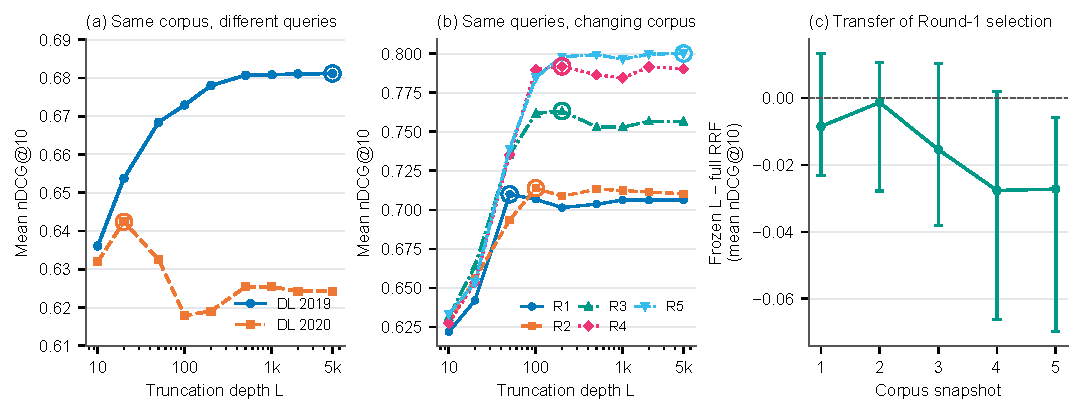
\includegraphics[width=\textwidth]{../../../figures/paper-v2/transfer.pdf}
\caption{Depth sensitivity and transfer. (a) Different queries on the same corpus. (b) The same queries across corpus snapshots, evaluated with each round's judgments. Circled points mark retrospectively selected best depths. (c) Round-1 depths applied to held-out queries across rounds. Error bars show nested bootstrap 95\% confidence intervals, including depth reselection and preserving query identities across rounds.}
\label{fig:transfer}\end{figure*}

\subsection{Fixed-K access cost}
\begin{table}[t]
\centering
\caption{Accesses to complete exact Top-20 under unit-access DiBud. All 770 queries complete.}
\label{tab:cost}
\small\setlength{\tabcolsep}{3pt}
\begin{tabular}{lrrrr}
\toprule
Query set & $n$ & Median & P95 & Maximum \\
\midrule
TREC-DL 2019 & 43 & 311 & 196410 & 3533518 \\
TREC-DL 2020 & 54 & 444 & 35562 & 211169 \\
NFCorpus & 323 & 308 & 2685 & 5035 \\
SciFact & 300 & 325 & 3362 & 5011 \\
TREC-COVID & 50 & 2544 & 56363 & 91290 \\
\bottomrule
\end{tabular}
\end{table}

A fixed result count does not stabilize access cost (Table~\ref{tab:cost}). On TREC-DL 2019, completing exact Top-20 takes a median of 311 accesses, but the P95 is 196410 and the maximum is 3533518: approximately 632 and 11362 times the median. The P95 is also 80 times the median on TREC-DL 2020 and 22 times on TREC-COVID. These differences motivate controlling accesses directly through a budget rather than indirectly through $K$.

\subsection{Certified output under equal budgets}
\begin{table}[t]
\centering
\caption{Mean certified output at $B=2048$. Both methods use unit accesses and the same certifier; only list selection differs.}
\label{tab:yield}
\small
\setlength{\tabcolsep}{3pt}
\begin{tabular}{lrrrr}
\toprule
& \multicolumn{2}{c}{Cap 100} & \multicolumn{2}{c}{Cap 20} \\ Query set & Balanced & DiBud & Balanced & DiBud \\
\midrule
TREC-DL 2019 & 41.86 & 46.19 & 17.77 & 17.91 \\
TREC-DL 2020 & 34.91 & 38.31 & 18.33 & 18.35 \\
NFCorpus & 62.06 & 63.71 & 19.24 & 19.28 \\
SciFact & 43.55 & 47.26 & 19.44 & 19.57 \\
TREC-COVID & 26.48 & 29.80 & 15.58 & 15.78 \\
\bottomrule
\end{tabular}
\end{table}

At $B=2048$, DiBud increases mean certified output within the first 100 positions from 41.77 to 45.05, a 7.86\% gain over Balanced (Table~\ref{tab:yield}). Within the first 20 positions, the mean changes from 18.07 to 18.18. All five sets gain output, with larger improvements for longer prefixes.
\begin{figure*}[t]
\centering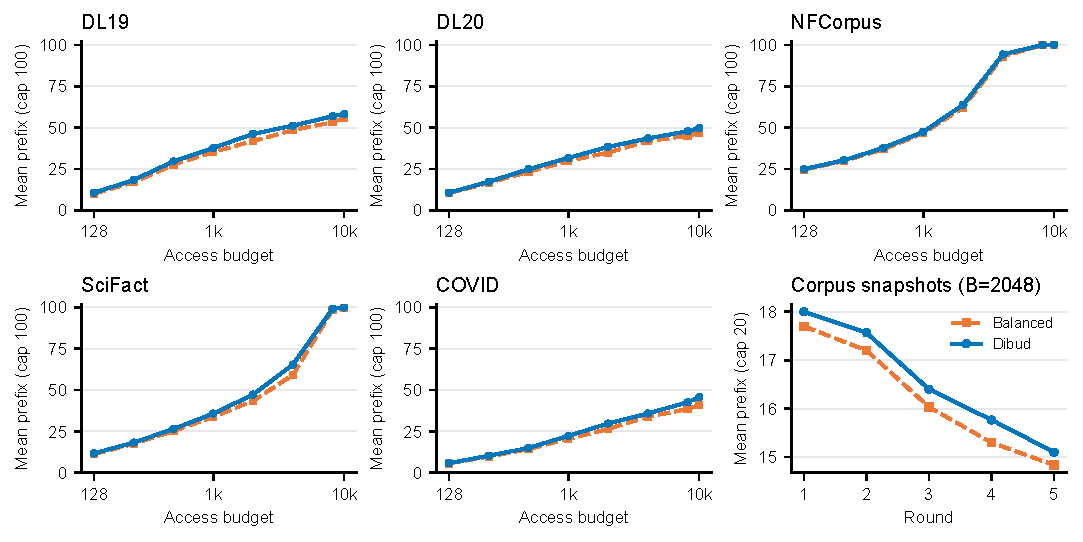
\includegraphics[width=\textwidth]{../../../figures/paper-v3/yield.pdf}
\caption{Certified output under equal budgets. Static panels cap output at 100; the snapshot panel uses a cap of 20 and $B=2048$. All plotted budget endpoints are observed.}
\label{fig:yield}\end{figure*}
Over the full log-budget range, DiBud has a larger normalized certified-prefix area than Balanced on all five static sets. The paired 95\% confidence intervals for these differences remain above zero with both unit accesses and batches of 64.

Across the five snapshots at $B=2048$, DiBud returns means of 18.00, 17.57, 16.40, 15.77, and 15.10 results within the first 20 positions, versus 17.70, 17.20, 16.03, 15.30, and 14.83 for Balanced. A fixed budget yields different output sizes as the corpus changes. DiBud improves the mean in every round. Full budget curves, output quantiles, empty-output rates, and delivery thresholds are retained with the experiment artifacts.

\subsection{Quality and access cost relative to exact Top-20}
We compare two stopping conditions on the same unit-SNRA trajectory: complete exact Top-20, or stop at the budget or at 20 certified results, whichever comes first. Evaluation uses linear-gain nDCG@20, with absent positions contributing zero. For each query set, five-fold calibration chooses the smallest budget retaining 90\%, 95\%, or 99\% of the reference mean nDCG@20; the frozen choice is evaluated on held-out queries. Retention is a ratio of means, not a mean of per-query ratios with an arbitrary value for zero-reference queries.
\begin{table}[H]
\centering
\caption{Held-out results after 95\% budget calibration. Retention is the ratio of mean nDCG@20; savings compare total accesses with completed exact Top-20.}
\label{tab:quality}
\small\setlength{\tabcolsep}{3pt}
\begin{tabular}{lrr}
\toprule
Query set & Retained (\%) & Fewer accesses (\%) \\
\midrule
TREC-DL 2019 & 95.05 & 99.53 \\
TREC-DL 2020 & 95.89 & 93.50 \\
NFCorpus & 95.81 & 65.92 \\
SciFact & 97.68 & 83.41 \\
TREC-COVID & 95.85 & 69.71 \\
\bottomrule
\end{tabular}
\end{table}

At the 95\% calibration target, held-out quality retention ranges from 95.05\% to 97.68\%, with 65.92\%--99.53\% fewer accesses across the five sets (Table~\ref{tab:quality}; Fig.~\ref{fig:quality}). TREC-DL 2019 retains 95.05\% of mean nDCG@20 while saving 99.53\% of accesses. Its large reduction reflects the cost of completing the long-tail queries in Section~3.3. Budgeted stopping preserves most of the measured relevance gain while avoiding much of this completion cost.
\begin{figure}[tbp]
\centering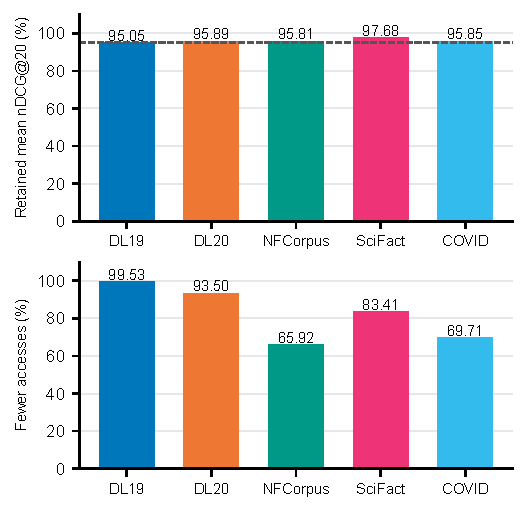
\includegraphics[width=\columnwidth]{../../../figures/paper-v3/quality-cost.pdf}
\caption{Held-out mean quality retention and access reduction relative to exact Top-20 after 95\% budget calibration. The dashed line marks the calibration target.}
\label{fig:quality}\end{figure}
At the 99\% target, five, four, and five calibration folds on TREC-DL 2019, TREC-DL 2020, and TREC-COVID do not reach the target within the tested budgets. Higher quality targets can require budgets beyond the evaluated range.
